\section{eo\-Time\-Counter Class Reference}
\label{classeo_time_counter}\index{eoTimeCounter@{eoTimeCounter}}
An {\bf eo\-Stat}{\rm (p.\,\pageref{classeo_stat})} that simply gives the user time since first generation It has to be tempatized by EOT because it must be an {\bf eo\-Stat}{\rm (p.\,\pageref{classeo_stat})}.  


{\tt \#include $<$eo\-Time\-Counter.h$>$}

Inheritance diagram for eo\-Time\-Counter::\begin{figure}[H]
\begin{center}
\leavevmode
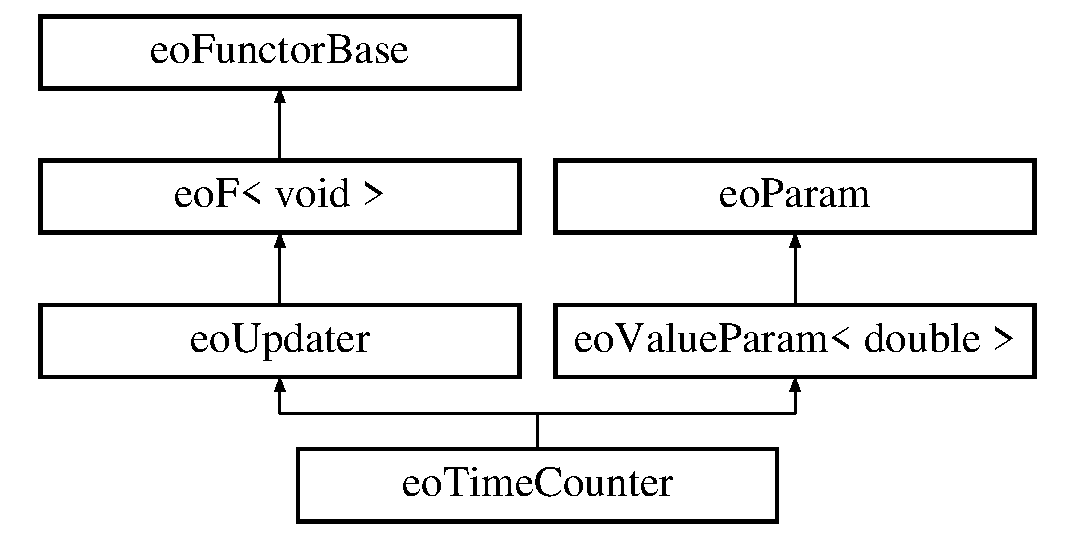
\includegraphics[height=4cm]{classeo_time_counter}
\end{center}
\end{figure}
\subsection*{Public Member Functions}
\begin{CompactItemize}
\item 
virtual void {\bf operator()} ()\label{classeo_time_counter_a1}

\begin{CompactList}\small\item\em simply stores the time spent in process in its {\bf value()}{\rm (p.\,\pageref{classeo_value_param_a2})} \item\end{CompactList}\end{CompactItemize}
\subsection*{Private Attributes}
\begin{CompactItemize}
\item 
clock\_\-t {\bf utime}\label{classeo_time_counter_r0}

\end{CompactItemize}


\subsection{Detailed Description}
An {\bf eo\-Stat}{\rm (p.\,\pageref{classeo_stat})} that simply gives the user time since first generation It has to be tempatized by EOT because it must be an {\bf eo\-Stat}{\rm (p.\,\pageref{classeo_stat})}. 



Definition at line 38 of file eo\-Time\-Counter.h.

The documentation for this class was generated from the following file:\begin{CompactItemize}
\item 
eo\-Time\-Counter.h\end{CompactItemize}
